\begin{figure}[H]
  \centering
  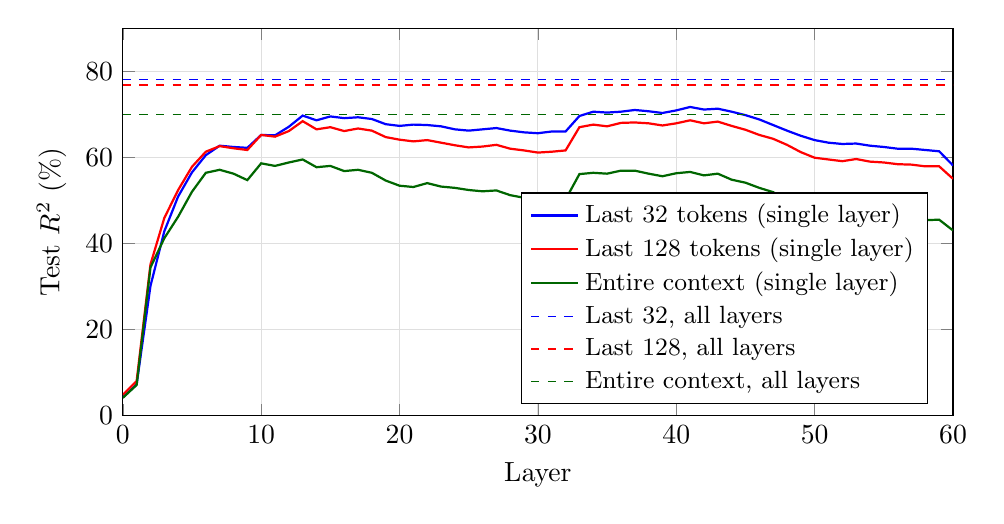
\begin{tikzpicture}
    \begin{axis}[
        width=\linewidth, height=6.5cm,
        xlabel={Layer}, ylabel={Test $R^2$ (\%)},
        xmin=0, xmax=60, ymin=0, ymax=90,
        xtick={0,10,20,30,40,50,60},
        grid=major, grid style={gray!25},
        legend pos=south east, legend cell align=left,
        legend style={font=\small},
      ]
      \addplot[thick, blue, mark=none] coordinates {
        (0,4.2) (1,7.2) (2,30.1) (3,42.8) (4,50.9) (5,56.5) (6,60.5) (7,62.7) (8,62.4) (9,62.2)
        (10,65.2) (11,65.1) (12,67.1) (13,69.7) (14,68.6) (15,69.5) (16,69.1) (17,69.3) (18,68.9) (19,67.7)
        (20,67.3) (21,67.6) (22,67.5) (23,67.2) (24,66.5) (25,66.2) (26,66.5) (27,66.8) (28,66.2) (29,65.8)
        (30,65.6) (31,66.0) (32,66.0) (33,69.6) (34,70.6) (35,70.4) (36,70.6) (37,71.0) (38,70.7) (39,70.3)
        (40,70.9) (41,71.7) (42,71.1) (43,71.3) (44,70.6) (45,69.8) (46,68.8) (47,67.5) (48,66.2) (49,65.0)
        (50,64.0) (51,63.4) (52,63.1) (53,63.2) (54,62.7) (55,62.4) (56,62.0) (57,62.0) (58,61.7) (59,61.4)
        (60,58.1)
      };
      \addlegendentry{Last 32 tokens (single layer)}
      \addplot[thick, red, mark=none] coordinates {
        (0,4.8) (1,8.0) (2,35.1) (3,45.9) (4,52.4) (5,57.8) (6,61.3) (7,62.6) (8,62.1) (9,61.7)
        (10,65.2) (11,64.8) (12,66.1) (13,68.4) (14,66.5) (15,67.0) (16,66.1) (17,66.7) (18,66.2) (19,64.7)
        (20,64.1) (21,63.7) (22,64.0) (23,63.4) (24,62.8) (25,62.3) (26,62.5) (27,62.9) (28,62.0) (29,61.6)
        (30,61.1) (31,61.3) (32,61.6) (33,67.0) (34,67.6) (35,67.2) (36,68.0) (37,68.1) (38,67.9) (39,67.4)
        (40,67.9) (41,68.6) (42,67.9) (43,68.3) (44,67.3) (45,66.4) (46,65.2) (47,64.3) (48,62.9) (49,61.2)
        (50,59.9) (51,59.5) (52,59.1) (53,59.6) (54,59.0) (55,58.8) (56,58.4) (57,58.3) (58,57.9) (59,57.9)
        (60,55.0)
      };
      \addlegendentry{Last 128 tokens (single layer)}
      \addplot[thick, black!60!green, mark=none] coordinates {
        (0,4.1) (1,7.1) (2,34.4) (3,41.2) (4,46.2) (5,52.0) (6,56.4) (7,57.1) (8,56.2) (9,54.7)
        (10,58.6) (11,58.0) (12,58.8) (13,59.5) (14,57.7) (15,58.0) (16,56.8) (17,57.1) (18,56.4) (19,54.6)
        (20,53.4) (21,53.1) (22,54.0) (23,53.2) (24,52.9) (25,52.4) (26,52.1) (27,52.3) (28,51.2) (29,50.6)
        (30,50.2) (31,50.3) (32,50.2) (33,56.1) (34,56.4) (35,56.2) (36,56.9) (37,56.9) (38,56.2) (39,55.6)
        (40,56.3) (41,56.6) (42,55.8) (43,56.2) (44,54.8) (45,54.1) (46,52.9) (47,51.9) (48,50.1) (49,48.1)
        (50,46.8) (51,46.2) (52,45.8) (53,46.5) (54,45.8) (55,45.9) (56,45.3) (57,45.5) (58,45.4) (59,45.5)
        (60,43.0)
      };
      \addlegendentry{Entire context (single layer)}
      \addplot[blue, dashed] coordinates {(0,78.0) (60,78.0)};
      \addlegendentry{Last 32, all layers}
      \addplot[red, dashed] coordinates {(0,76.8) (60,76.8)};
      \addlegendentry{Last 128, all layers}
      \addplot[black!60!green, dashed] coordinates {(0,69.9) (60,69.9)};
      \addlegendentry{Entire context, all layers}
    \end{axis}
  \end{tikzpicture}
  \caption{Test $R^2$ for decoding past difficulty (mean surprisal of the last 32 or 128 tokens, or of the entire context so far) from a linear probe on one layer's activations at the current token. Dashed: one probe on all 61 layers. Single layers peak at layer 41 (32), 41 (128) and 13 (entire context).}
  \label{fig:layer-r2-past}
\end{figure}
